%%%%%%%%%%%%%%%%%%%%%%%%%%%%%%%%%%%%%%%%%%%%%%%%%%%%%%%%%%%%%%%%%%%%%%%%%%%%%%%%%%
\begin{frame}[fragile]\frametitle{}
\begin{center}
{\Large Introduction}
\end{center}
\end{frame}


%%%%%%%%%%%%%%%%%%%%%%%%%%%%%%%%%%%%%%%%%%%%%%%%%%%%%%%%%%%%%%%%%%%%%%%%%%%%%%%%%%%
\begin{frame}[fragile]\frametitle{Quote}
\begin{lstlisting}
"I always hope that when I start looking at a new language, there will be some mind-opening new ideas to find, and Swift definitely doesn't disappoint. Swift tries to be expressive, flexible, concise, safe, easy to use, and fast. Most languages compromise significantly in at least one of these areas."

- Jeremy Howard
\end{lstlisting}
\end{frame}

%%%%%%%%%%%%%%%%%%%%%%%%%%%%%%%%%%%%%%%%%%%%%%%%%%%%%%%%%%%%%%%%%%%%%%%%%%%%%%%%%%%
\begin{frame}[fragile]\frametitle{Quote}
\begin{lstlisting}
"PyTorch was created to overcome the gaps in Tensorflow. FastAI was built to fill gaps in tooling for PyTorch. But now we're hitting the limits of Python, and Swift has the potential to bridge this gap"

- Jeremy Howard
\end{lstlisting}
\end{frame}

%%%%%%%%%%%%%%%%%%%%%%%%%%%%%%%%%%%%%%%%%%%%%%%%%%%%%%%%%%%
\begin{frame} \frametitle{What is Swift?}
\begin{itemize}
\item Swift is fast, as close to C as possible
\item Swift is simple and readable, very similar to Python. 
\item Swift is a more efficient, stable and secure programming language as compared to Python.
\item Swift is good for Mobile Apps development, official language for iOS apps.
\item Swift has strong integrated support for automatic differentiation.
\item Swift lets seamlessly import libraries from Python like NumPy, pandas, matplotlib and scikit-learn. 
\item Swift has support from Apple, Google and FastAI.
\end{itemize}
\end{frame}

%%%%%%%%%%%%%%%%%%%%%%%%%%%%%%%%%%%%%%%%%%%%%%%%%%%%%%%%%%%%%%%%%%%%%%%%%%%%%%%%%%%
\begin{frame} \frametitle{Swift Ecosystem}
\begin{center}
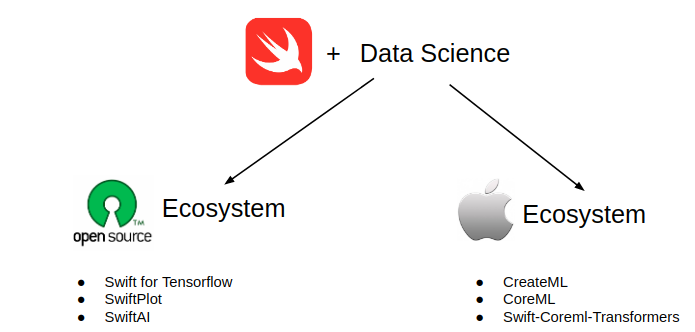
\includegraphics[width=0.9\linewidth,keepaspectratio]{s4tf2}
\end{center}

\begin{itemize}
\item Open-Source Swift can be downloaded and run on any machine,
\item For Apple ecosystem, you need to have an Apple machine to work on and you can only build for Apple devices like the iOS, macOS etc.
\end{itemize}

\end{frame}

%%%%%%%%%%%%%%%%%%%%%%%%%%%%%%%%%%%%%%%%%%%%%%%%%%%%%%%%%%%%%%%%%%%%%%%%%%%%%%%%%%%
\begin{frame} \frametitle{iOS/MacOS ML Apps}
\begin{center}
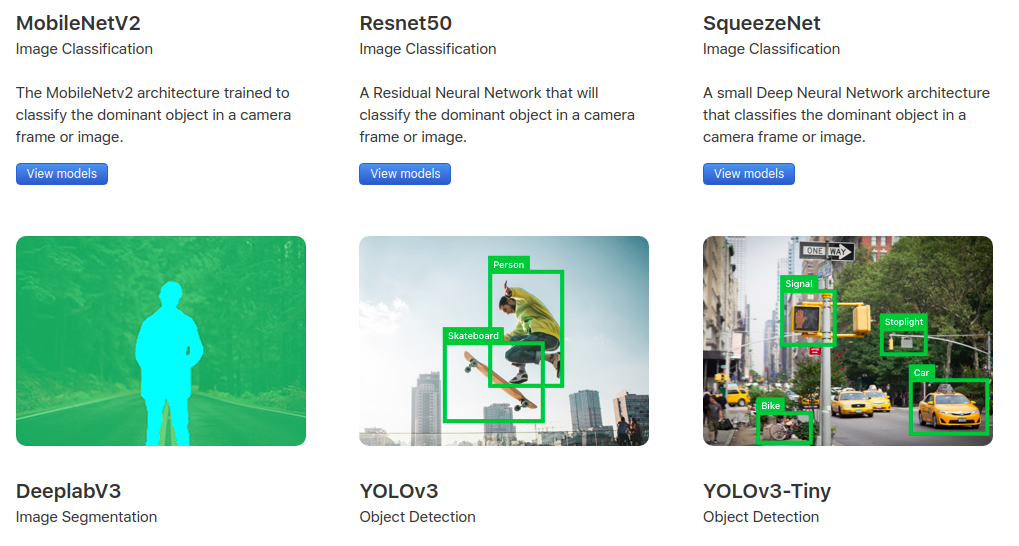
\includegraphics[width=0.9\linewidth,keepaspectratio]{s4tf3}
\end{center}
\end{frame}



%%%%%%%%%%%%%%%%%%%%%%%%%%%%%%%%%%%%%%%%%%%%%%%%%%%%%%%%%%%%%%%%%%%%%%%%%%%%%%%%%%%
\begin{frame} \frametitle{What is Swift for Tensorflow?}
\begin{center}

\includegraphics[width=0.65\linewidth,keepaspectratio]{s4tf1}
\end{center}
\end{frame}


%%%%%%%%%%%%%%%%%%%%%%%%%%%%%%%%%%%%%%%%%%%%%%%%%%%%%%%%%%%%%%%%%%%%%%%%%%%%%%%%%%
\begin{frame}[fragile]\frametitle{}
\begin{center}
{\Large Getting Started}
\end{center}
\end{frame}

%%%%%%%%%%%%%%%%%%%%%%%%%%%%%%%%%%%%%%%%%%%%%%%%%%%%%%%%%%%
\begin{frame} \frametitle{Installation on Windows}
\begin{itemize}
\item NO NEED TO Download RELEASE toolchain and sig from https://swift.org/download/ but get it from "Development Snapshots" of Windows from https://github.com/tensorflow/swift/blob/master/Installation.md

\item \lstinline|gpg.exe --import all-keys.asc| from https://swift.org/keys/all-keys.asc
\item Install exe
\item It gets installed in \lstinline|C:\\Library\\Developer\\Toolchains|
\item Define SDKROOT in Env Variables (..shown in next slide)
\end{itemize}

{\tiny (Note:  The .exe installer for Windows are signed using GnuPG with one of the keys of the Swift open source project. Everyone is strongly encouraged to verify the signatures before using the software.). For Other OSs refer https://swift.org/getting-started/\#installing-swift}
\end{frame}

%%%%%%%%%%%%%%%%%%%%%%%%%%%%%%%%%%%%%%%%%%%%%%%%%%%%%%%%%%%
\begin{frame} \frametitle{Installation on Windows}
\begin{itemize}

\item From an (elevated) "Administrator" x64 Native Tools for VS2019 Command Prompt shell (Follow step 4 mentioned in link above)
\item Set \lstinline|SDKROOT=C:/Library/Developer/Platforms/| \lstinline|Windows.platform/Developer/SDKs/Windows.sdk|
\item Create test.swift with code as \lstinline|print("hello")| and run
\item \lstinline|swiftc -sdk \%SDKROOT\% -I \%SDKROOT\%/usr/lib/swift -L \%SDKROOT\%/usr/lib/swift/windows -emit-executable -o test.exe test.swift|
\item \lstinline|test.exe|
\end{itemize}
{\tiny (Note:  Interpreter mode and direct invocation from VS 2019 are currently not supported on Windows.. Ref: https://github.com/tensorflow/swift/blob/master/Installation.md)}
\end{frame}